\section{九点圆与欧拉线}
\subsection{九点圆}
\begin{definition}
    $\triangle ABC$三条高的垂足、三边中点,以及垂心与顶点的三条连线段中点,这九点共圆。
\end{definition}
\begin{figure}[htbp]
    \centering
    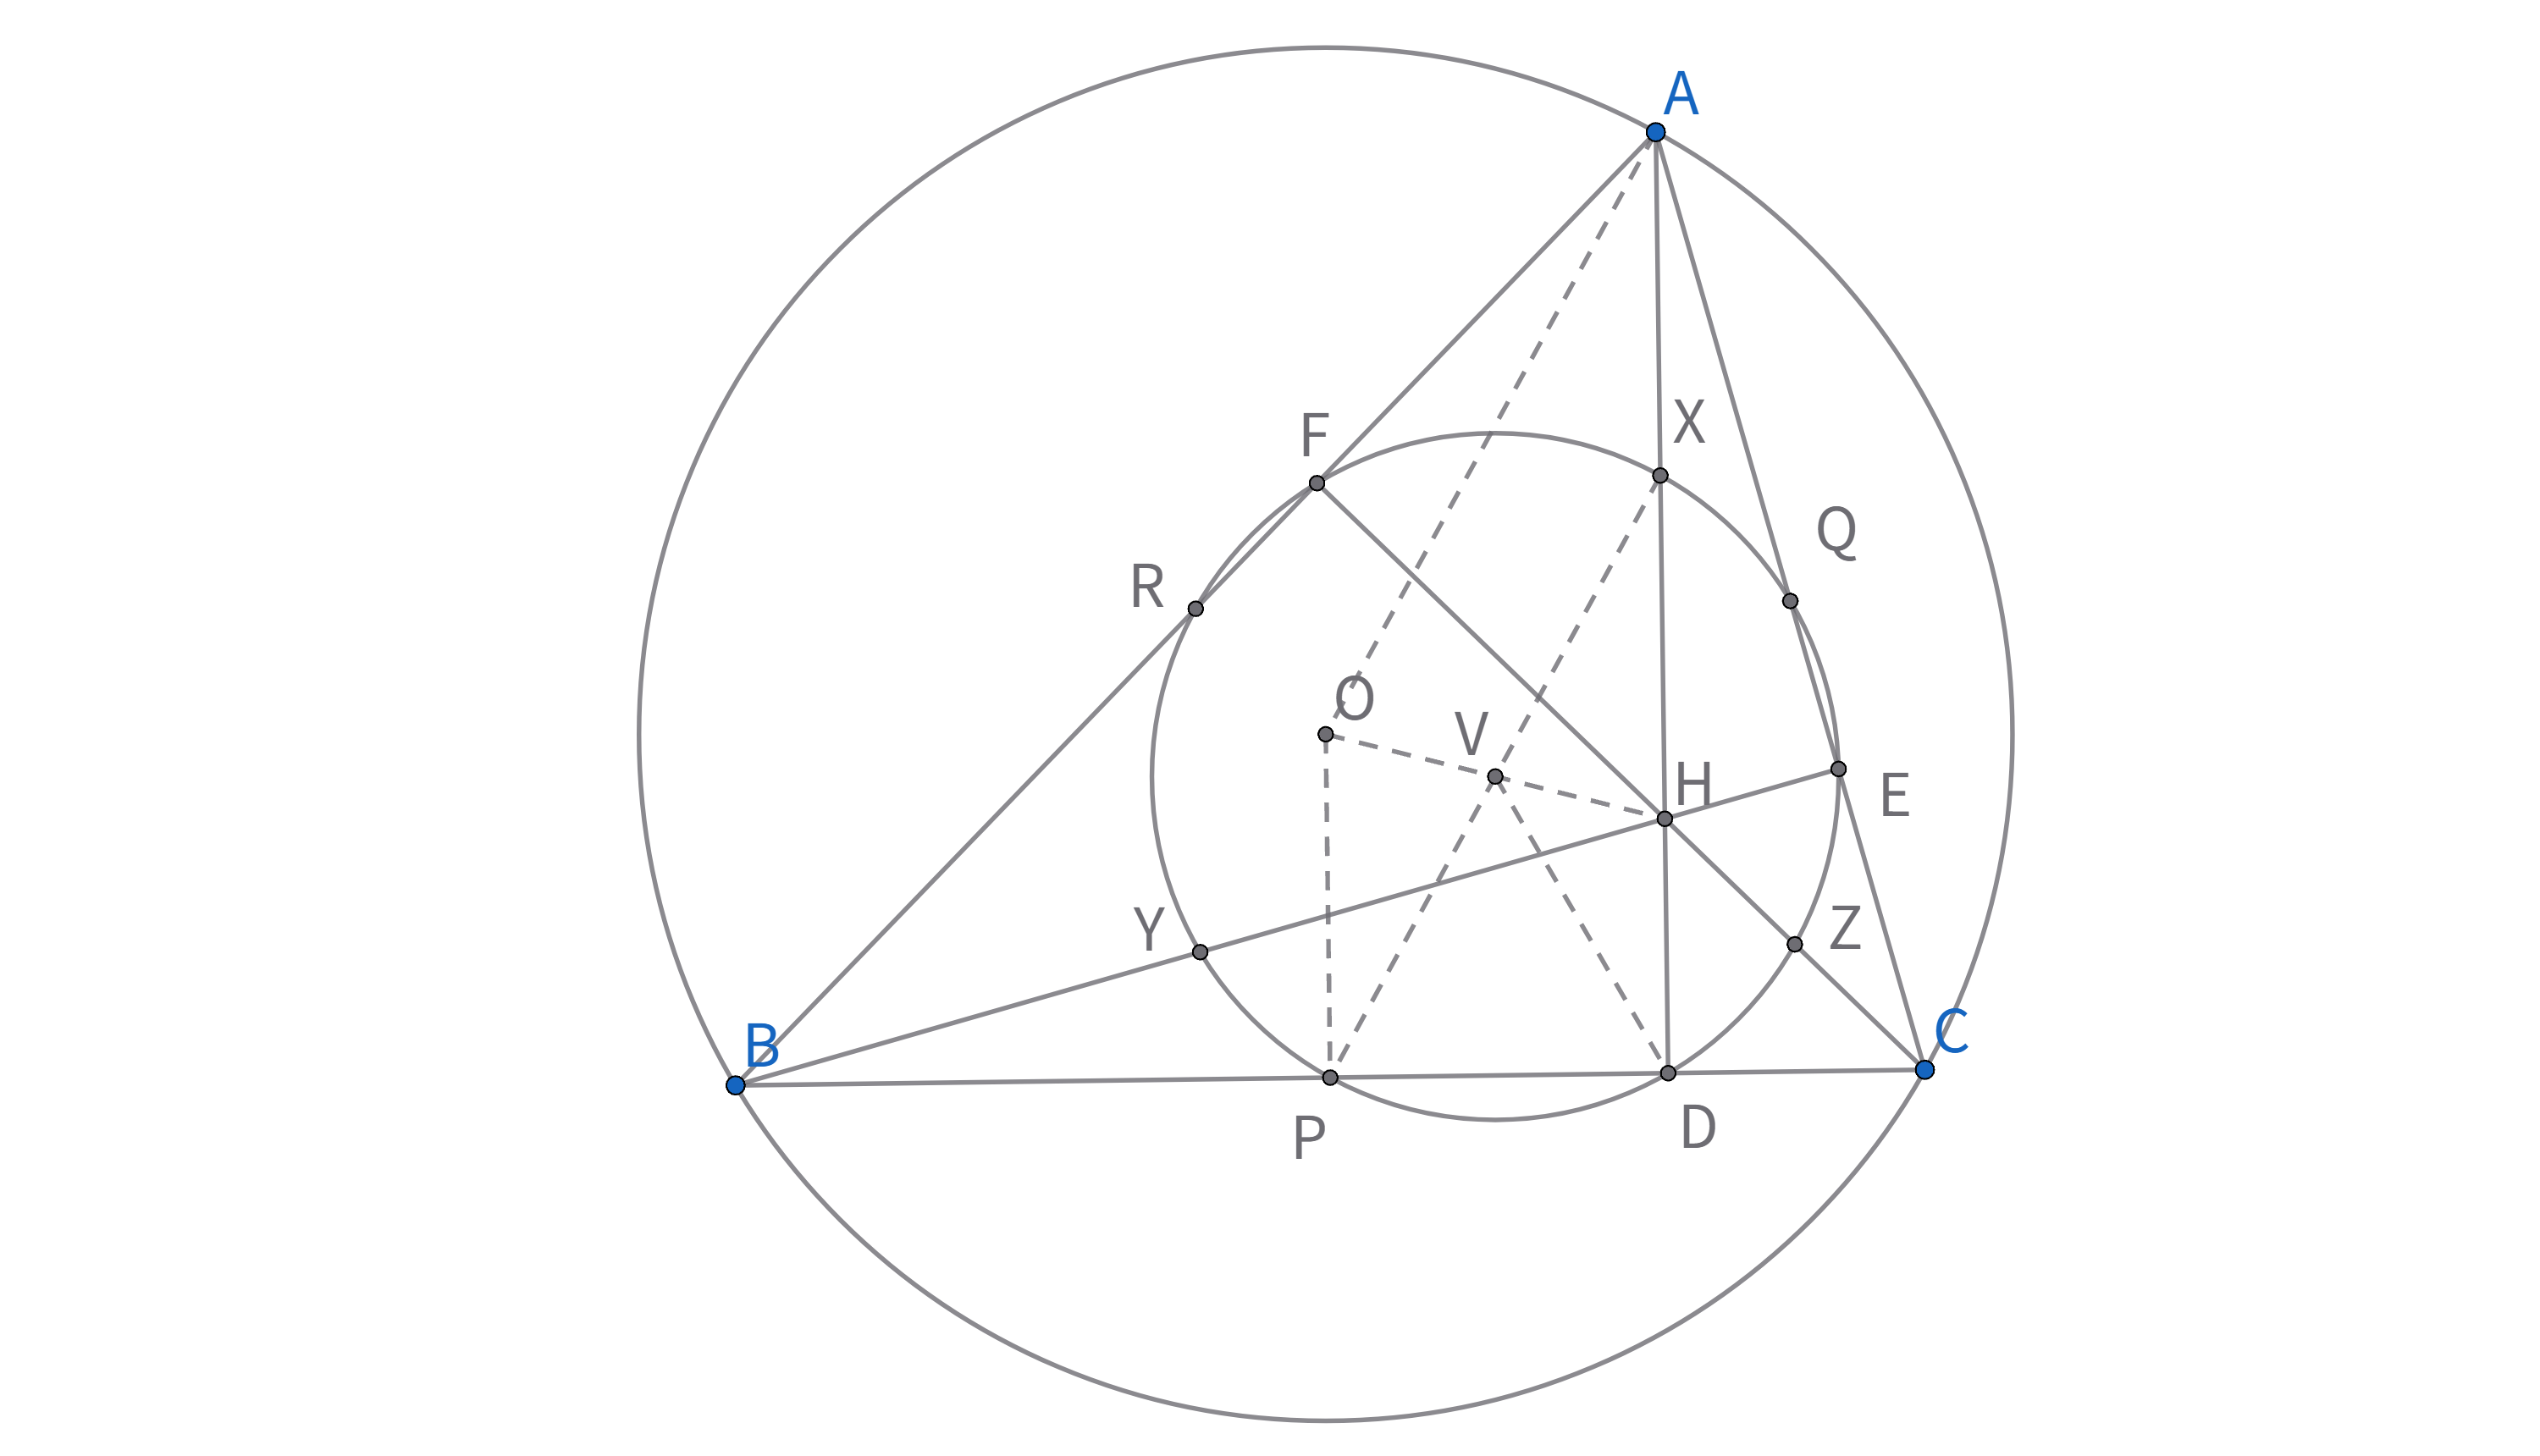
\includegraphics[width=\linewidth]{figures/九点圆辅助线.png}
    \caption{九点圆}
\end{figure}
\begin{proposition}[九点圆性质]
    九点圆具有如下性质:\\
    (1) 九点圆的半径是三角形的外接圆半径之半。\\
    (2) 九点圆的圆心恰为垂心与外心连线的中点。\\
    (3) 三角形的九点圆与其外接圆是以垂心为外位似中心,位似比为1:2的位似形;垂心与外接圆上任一点的连线段被九点圆截成相等的两部分。\\
    (4) 三角形的九点圆与其外接圆是以重心为内位似中心,位似比为1:2的位似形。\\
\end{proposition}
% (3)三角形的九点圆与三角形的内切圆,三个旁切圆均相切(费尔巴哈定理),

\newpage 
\subsection{欧拉线}
\begin{theorem}
    $\triangle ABC$的外心O,重心G,垂心H,九点圆圆心V四点共线。并且
    $$
    \frac{OG}{GH}=\frac{1}{2},\quad 
    \frac{GV}{VH}=\frac{1}{3}.
    $$
\end{theorem}
\begin{figure}[htbp]
    \centering
    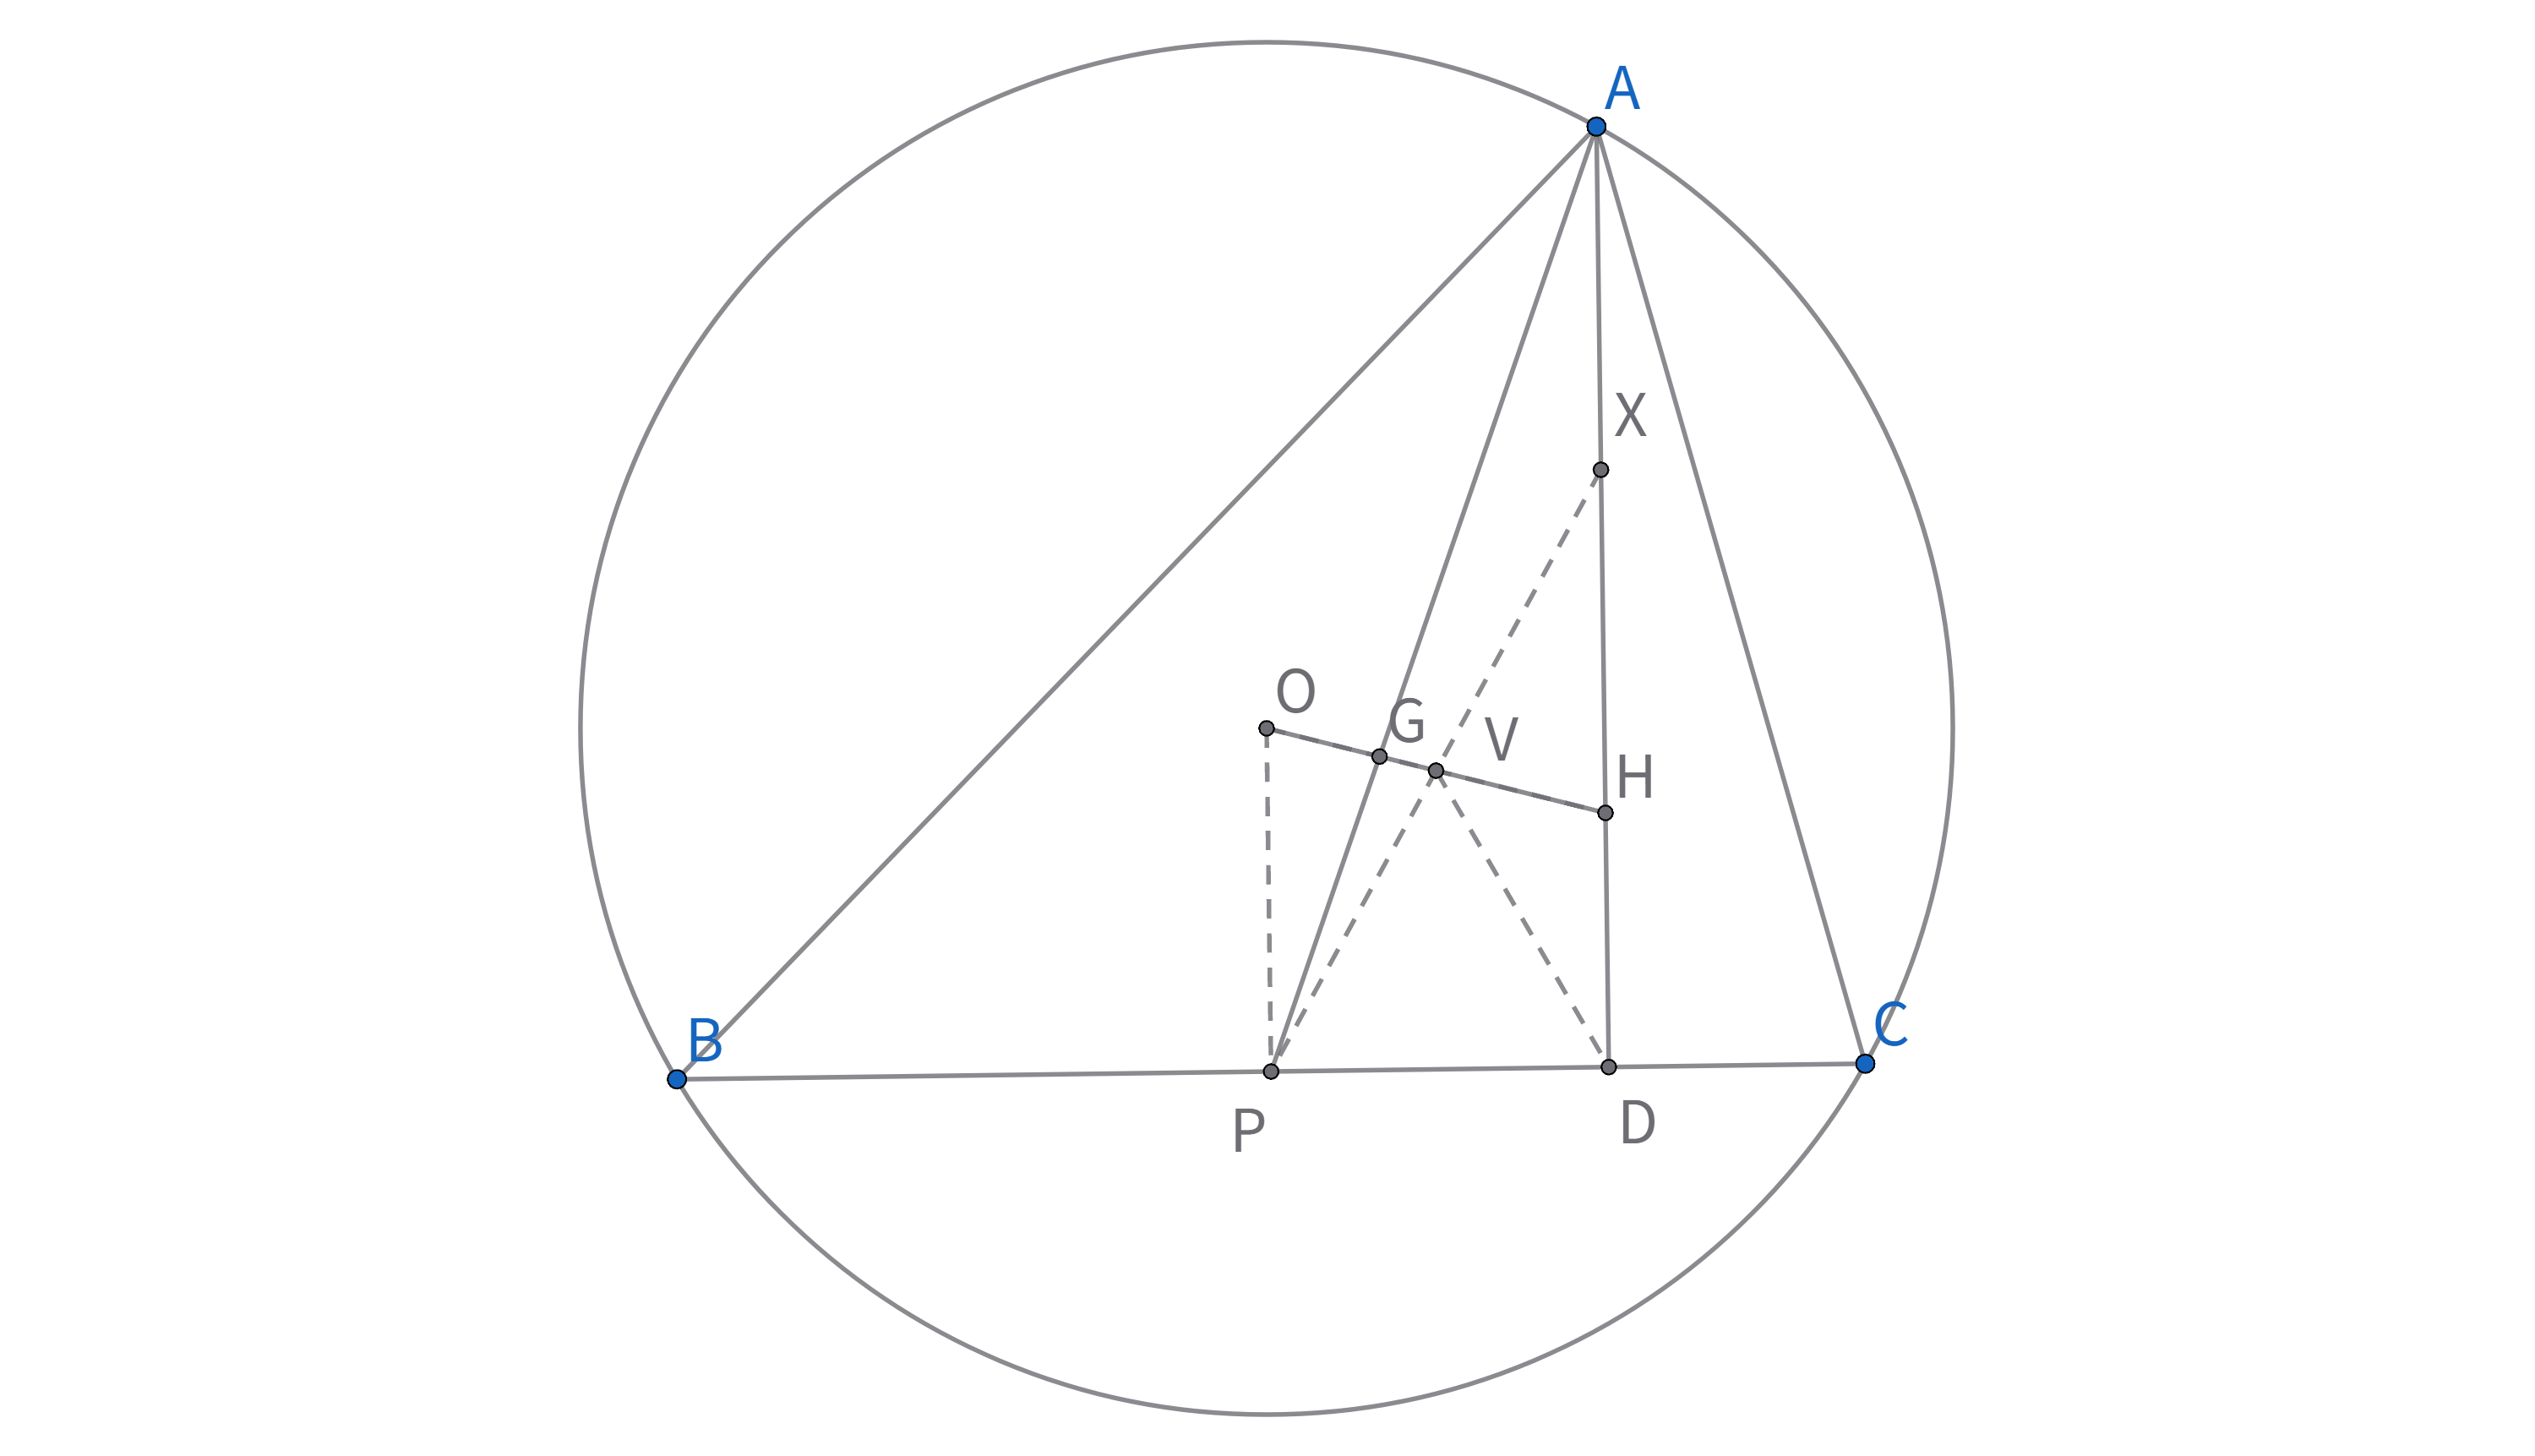
\includegraphics[width=\linewidth]{figures/欧拉线.png}
    \caption{欧拉线}
\end{figure}